\section{Fair Value Modeling}

\subsection*{Motivation}

Investment-grade CDS spreads reflect the market's assessment of corporate
default risk and the compensation demanded for bearing that risk. Conceptually,
the main drivers of IG spreads can be grouped into three channels:

\begin{itemize}
  \item \textbf{Risk appetite and equity markets.} Equity indices are a
    real-time proxy for growth expectations and investor risk appetite. When
    equities decline, the implied probability of corporate distress rises, and
    credit spreads widen. The S\&P 500 captures this channel for US-domiciled
    names.

  \item \textbf{Implied volatility.} The VIX measures the cost of hedging
    equity tail risk. Higher implied volatility signals greater uncertainty
    about future cash flows and asset values, which directly increases the
    credit risk premium embedded in IG spreads.

  \item \textbf{Rates and monetary policy.} Treasury yields and the shape of
    the yield curve affect corporate funding costs, discount rates, and the
    macroeconomic outlook. The 10-year yield (UST10) captures the level of
    long-term rates, the 2s--10s curve (USYC) captures term-structure slope
    and recession expectations, and SOFR captures the stance of near-term
    monetary policy. Together, these variables span the rates environment that
    IG issuers face.
\end{itemize}

A model combining these three channels should capture the principal macro forces
acting on CDX IG without including other credit indices (such as CDX HY) as
regressors, which would make the model largely tautological.

\subsection*{Model comparison and best specification}

Several candidate OLS models were estimated on daily changes
(\(\Delta CDXIG\)) and ranked by out-of-sample performance. For each model, a
single set of coefficients is estimated on the first 80\% of the sample
(training set) and held fixed; the remaining 20\% serves as an out-of-sample
test set on which the model is evaluated with no re-estimation. This static
coefficient approach provides a clean assessment of model stability but assumes
that the relationships between CDX IG and its drivers remain constant over
time---an assumption we relax in the sensitivity document, where a
rolling-window alternative is also examined. The best-performing static
specification is:

\[
\Delta CDXIG_t = \alpha + \gamma_1 \Delta VIX_t + \gamma_2 \Delta S\&P_t
  + \gamma_3 \Delta UST10_t + \gamma_4 \Delta USYC_t
  + \gamma_5 \Delta SOFR_t + u_t
\]

Key results:
\begin{itemize}
  \item Out-of-sample \(R^2 \approx 0.698\) and RMSE \(\approx 1.60\) (in
    daily spread-change units).
  \item Predicted daily changes are integrated from the initial observed level
    to reconstruct a model-implied fair-value path for CDX IG.
  \item Residual dislocations (observed minus fair value): the 95th percentile
    absolute residual is approximately 27\,bps, with 60 flagged observations
    exceeding that threshold.
\end{itemize}

The fact that this specification---spanning risk appetite, volatility, and the
rates complex---achieves nearly 70\% out-of-sample explanatory power confirms
that IG credit spreads are primarily a function of broad macro risk factors
rather than idiosyncratic credit events over this sample.

\subsection*{Practical applications}

\begin{itemize}
  \item \textbf{Dislocation screening:} residual z-scores identify periods
    where observed spreads deviate materially from macro-implied fair value,
    which may signal mean-reversion opportunities or structural breaks.
  \item \textbf{Scenario analysis:} the model can be stressed under
    hypothetical rate, equity, or volatility shocks to estimate the expected
    impact on CDX IG spreads.
  \item \textbf{Regime conditioning:} model robustness could be further
    improved by introducing regime indicators (e.g.\ high-volatility vs.\
    low-volatility environments) to allow coefficients to vary across market
    states.
\end{itemize}

Four candidate specifications were tested, each targeting a distinct
transmission channel:

\begin{description}
  \item[RatesVolEquity\_d] \(\Delta VIX\), \(\Delta S\&P\), \(\Delta UST10\),
    \(\Delta USYC\), \(\Delta SOFR\) --- combines equity risk appetite, implied
    volatility, and the US rates complex.
  \item[CrossMarket\_d] \(\Delta ITRX\;IG\), \(\Delta ITRX\;XO\),
    \(\Delta ESTX600\), \(\Delta EURUSD\), \(\Delta DEM10\) --- captures
    European credit and equity cross-market spillovers together with the
    EUR/USD exchange rate and German sovereign yields.
  \item[InflationMacro\_d] \(\Delta CO\), \(\Delta US5BEI\),
    \(\Delta UST2\), \(\Delta DEM2\) --- focuses on inflation expectations
    (via crude oil and the US breakeven rate) and short-end government yields.
    FR5BEI is excluded due to insufficient data coverage (see sensitivity
    document, Section~2).
  \item[FXBasisPolicy\_d] \(\Delta EURUSD\), \(\Delta EURUSD\;3m\;BS\),
    \(\Delta SOFR\), \(\Delta ESTR\), \(\Delta DEYC\) --- emphasises
    cross-currency funding conditions and central-bank policy rates.
\end{description}

\begin{figure}[H]
  \centering
  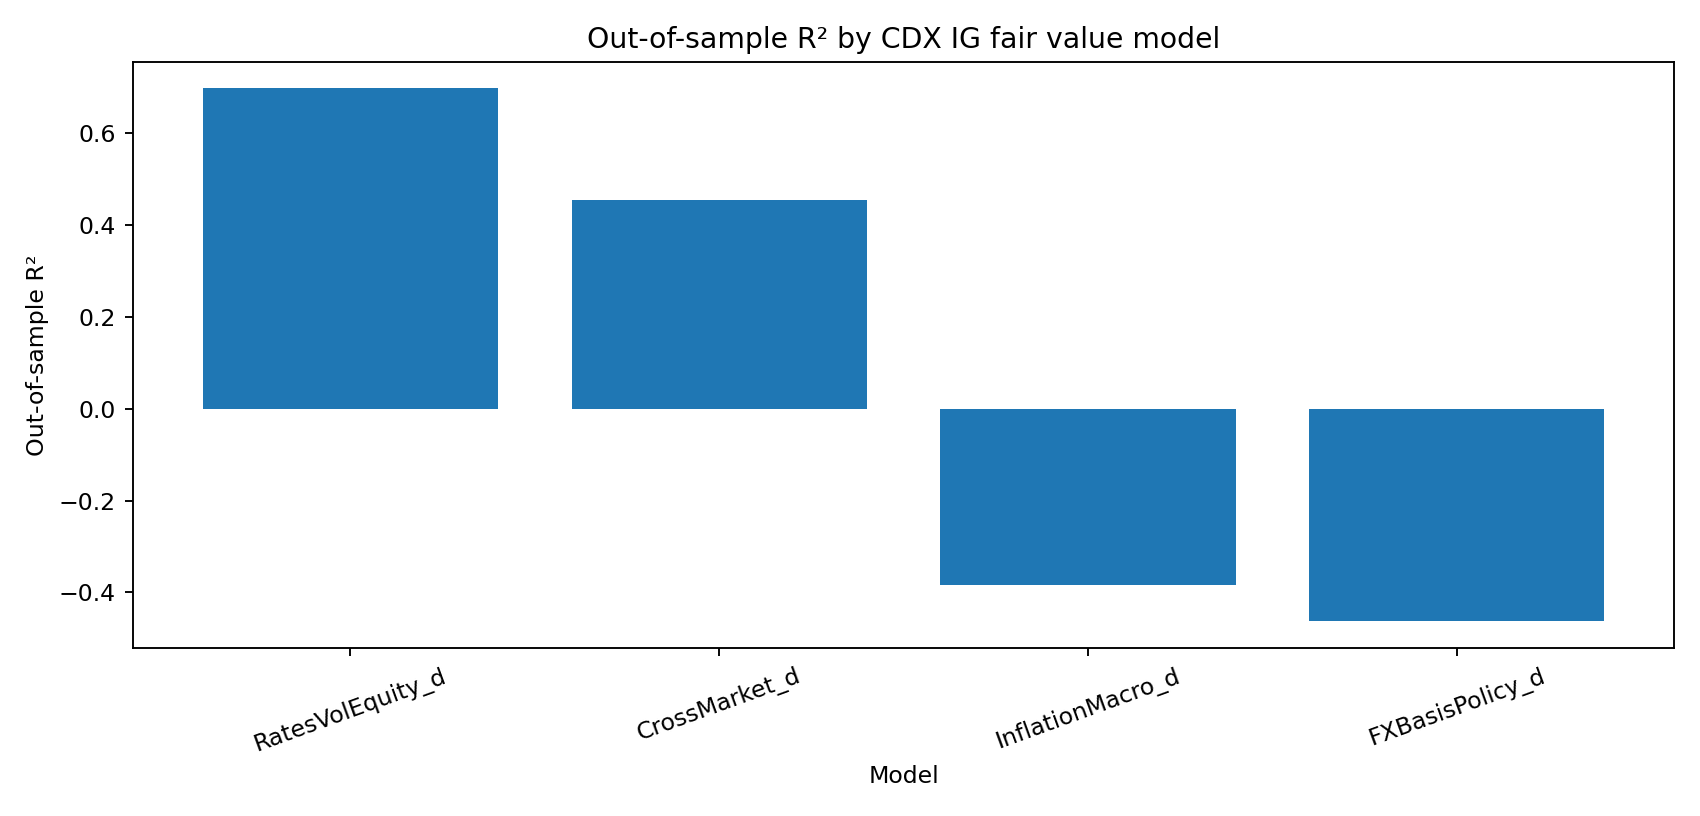
\includegraphics[width=\textwidth]{../../../output/figures/CDX_IG_fair_value_model_comparison.png}
  \caption{Out-of-sample \(R^2\) comparison across alternative CDX IG fair-value models.}
\end{figure}

\begin{figure}[H]
  \centering
  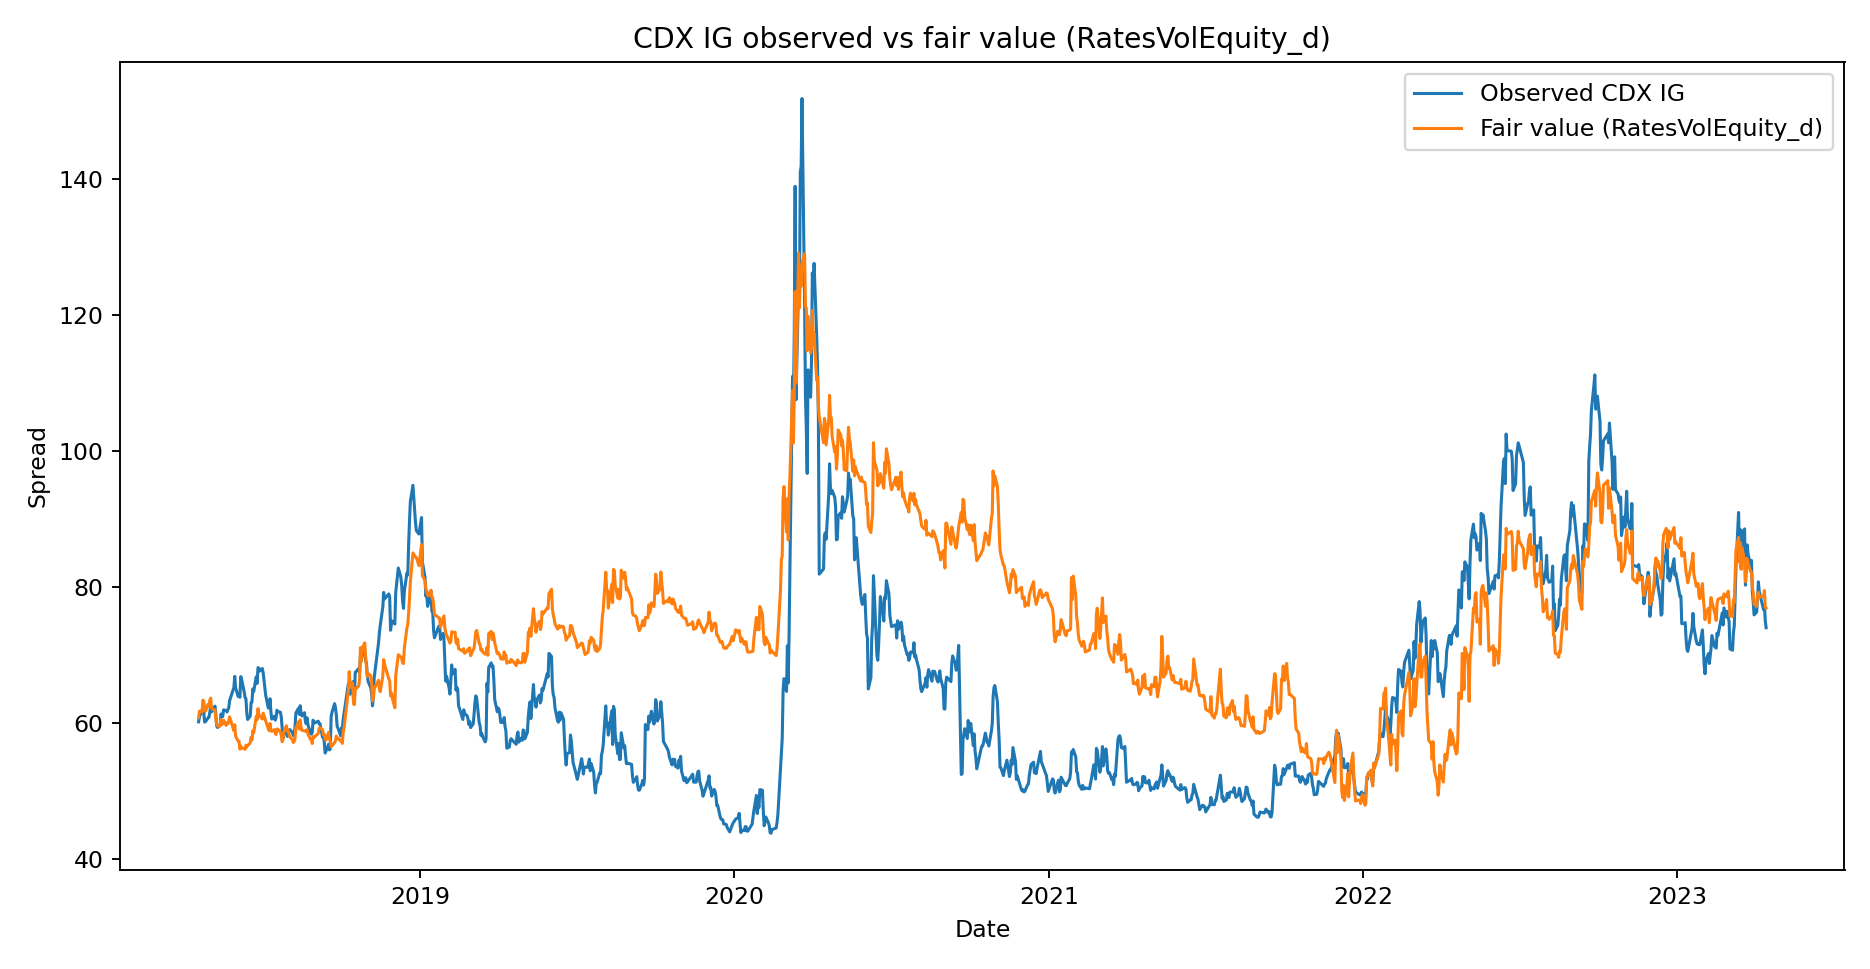
\includegraphics[width=\textwidth]{../../../output/figures/CDX_IG_fair_value_best_model.png}
  \caption{Observed CDX IG vs fair-value level implied by the best change-based model.}
\end{figure}
